% main.tex  — AITL on Space (camera-ready minimal example)
\documentclass[conference]{IEEEtran}

% ---------- Fonts & math ----------
\usepackage{newtxtext,newtxmath} % Times系 (TU対応) で LuaHBTeX 警告回避
\usepackage{amsmath,amssymb}
\usepackage{siunitx}
\sisetup{detect-all=true}

% ---------- Graphics & colors ----------
\usepackage{graphicx,xcolor,booktabs}
\usepackage{tikz}
\usetikzlibrary{positioning,arrows.meta,shapes.geometric,shapes.misc,shapes.multipart,fit}

% ---------- Links ----------
\usepackage[hidelinks]{hyperref}

% ---------- Helpers ----------
\usepackage{placeins} % \FloatBarrier
\renewcommand{\arraystretch}{1.1}

% ---------- Title ----------
\title{AITL on Space: A Robust Three-Layer Architecture\\
with a Tri-NVM Hierarchy (SRAM\,/\,MRAM\,/\,FRAM)\\
for Long-Duration Spacecraft Autonomy}

\author{\IEEEauthorblockN{Shinichi Samizo}
\IEEEauthorblockA{Independent Semiconductor Researcher\\
Former Engineer at Seiko Epson Corporation\\
Email: \texttt{shin3t72@gmail.com}\quad GitHub: \href{https://github.com/Samizo-AITL}{github.com/Samizo-AITL}}
}

\begin{document}
\maketitle

\begin{abstract}
We propose \emph{AITL on Space}, a three-layer robust control architecture (Robust Core, FSM Supervisor, AI Adaptor) implemented on a 22\,nm FDSOI SoC with a hardened tri-NVM hierarchy (SRAM/MRAM/FRAM). The system targets ultra-robust autonomy under radiation, thermal cycling, and long-term drift. This paper outlines the architecture, an 11D state-space plant model (8--20D extensible), an $H_\infty$ mixed-sensitivity design flow, and a verification pipeline from FPGA HIL to ASIC.
\end{abstract}

\section{Introduction}
Long-duration missions require high availability under total ionizing dose (TID), single event effects (SEE), and thermal cycles. Conventional PID\,+\,Flash architectures face reliability limits due to charge-trap drift and write endurance. We summarize related work and motivate AITL on Space as a resilient alternative.

\section{System Architecture}
AITL comprises three layers:
\begin{itemize}
\item \textbf{Robust Core} for $H_\infty$/MPC/SMC control,
\item \textbf{FSM Supervisor} (Safe/Nominal/Recovery; FDI/FDII),
\item \textbf{AI Adaptor} for long-term re-identification and drift compensation.
\end{itemize}
A tri-NVM hierarchy is adopted: SRAM for execution, MRAM for code/logs (ECC\,+\,scrub, A/B slots), and FRAM for safe boot and FSM state. The target implementation is a 22\,nm FDSOI SoC hardened for radiation and temperature cycling.

% ===== Figure 1: Architecture =====
\begin{figure}[t]
\centering
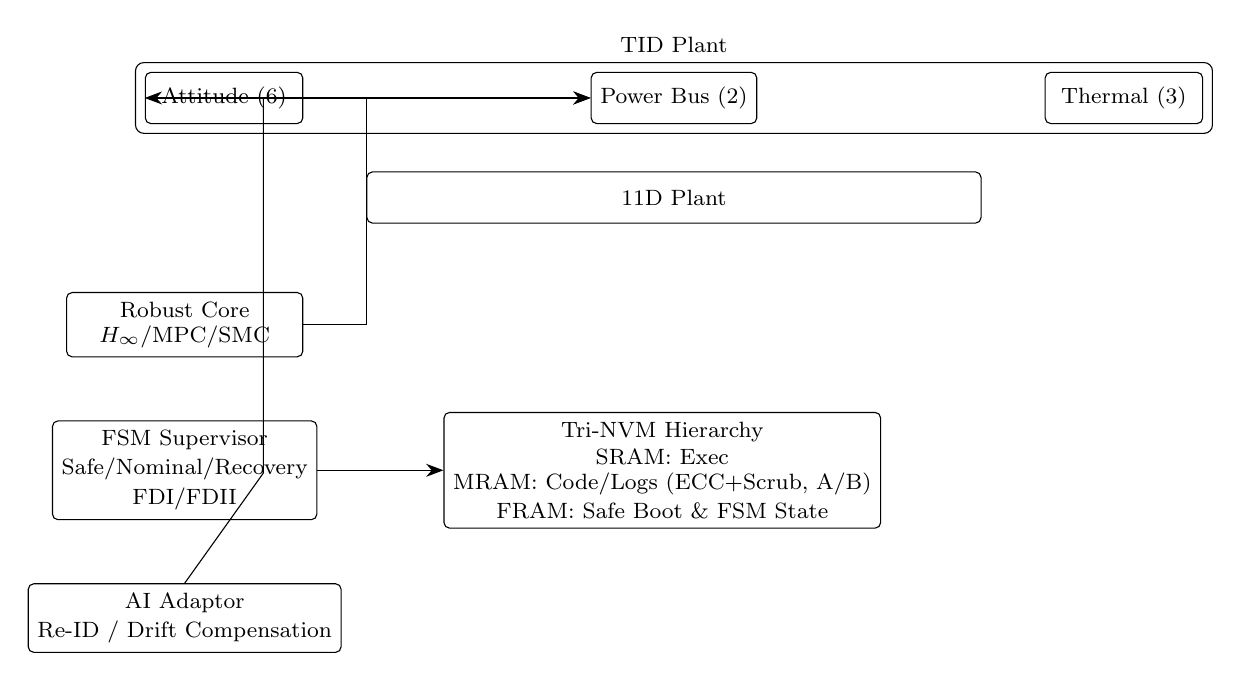
\begin{tikzpicture}[
  node distance=6mm and 8mm,
  box/.style={draw, rounded corners=2pt, minimum width=30mm, minimum height=6.5mm, align=center, font=\footnotesize},
  small/.style={draw, rounded corners=2pt, minimum width=20mm, minimum height=6.5mm, align=center, font=\footnotesize},
  >={Stealth[length=2.2mm]}
]
% Plant blocks
\node[box, minimum width=78mm] (plant) {11D Plant};
\node[small, above left=of plant] (att) {Attitude (6)};
\node[small, above=of plant] (bus) {Power Bus (2)};
\node[small, above right=of plant] (thm) {Thermal (3)};

% Left column
\node[box, below left=12mm and 8mm of plant.west] (core)
  {\shortstack{Robust Core\\ $H_\infty$/MPC/SMC}};
\node[box, below=8mm of core] (fsm)
  {\shortstack{FSM Supervisor\\ Safe/Nominal/Recovery\\ FDI/FDII}};
\node[box, below=8mm of fsm] (ai)
  {\shortstack{AI Adaptor\\ Re-ID / Drift Compensation}};

% Right NVM
\node[box, right=16mm of fsm, minimum width=55mm, anchor=west] (nvm)
  {\shortstack{Tri-NVM Hierarchy\\
  SRAM: Exec\\
  MRAM: Code/Logs (ECC+Scrub, A/B)\\
  FRAM: Safe Boot \& FSM State}};

% Wires
\draw[->] (core.east) -- ++(8mm,0) |- (att.west);
\draw[->] (core.east) -- ++(8mm,0) |- (bus.west);
\draw[->] (fsm.east) -- (nvm.west);
\draw[->] (ai.north) -- ++(10mm,14mm) |- (bus.west);

% plant grouping frame
\node[draw, rounded corners=3pt, fit=(att)(bus)(thm), label={[font=\footnotesize]above:TID Plant}] (plantfit) {};
\end{tikzpicture}
\caption{AITL on Space architecture with Robust Core, Supervisor FSM, AI Adaptor, and the Tri-NVM hierarchy.}
\label{fig:arch}
\end{figure}

\section{Mathematical Model}
We use an 11D discrete-time plant that couples attitude (6), power bus (2), and thermal nodes (3):
\begin{align}
  x_{k+1} &= A x_k + B u_k + E w_k, \label{eq:state}\\
  y_k     &= C x_k + D u_k + v_k. \label{eq:output}
\end{align}
The model extends to 20D by adding translational axes and bias states. $w_k$ and $v_k$ represent disturbance and sensor noise, respectively.

% ===== Figure 2: Control loop =====
\begin{figure}[t]
\centering
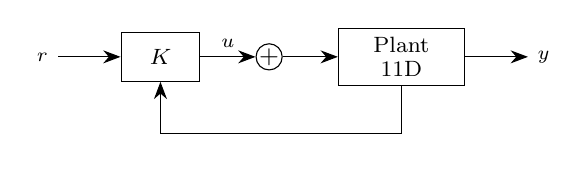
\begin{tikzpicture}[
  node distance=8mm and 8mm,
  sum/.style={circle, draw, inner sep=0pt, minimum size=3.3mm},
  blk/.style={draw, minimum width=10mm, minimum height=6.2mm, align=center, font=\footnotesize},
  >={Stealth[length=2.2mm]}
]
\node[blk] (k) {$K$};
\node[sum, right=7mm of k] (s) {\small $+$};
\node[blk, right=7mm of s, minimum width=16mm] (p) {\shortstack{Plant\\ 11D}};
\draw[->] (k) -- node[above, font=\scriptsize] {$u$} (s);
\draw[->] (s) -- (p);
\draw[<-] (k.west) -- ++(-8mm,0) node[left, font=\scriptsize] {$r$};
\draw[->] (p.east) -- ++(8mm,0) node[right, font=\scriptsize] {$y$};
\draw[->] (p.south) |- ++(0,-6mm) -| node[pos=0.25, below, font=\scriptsize] {} (k.south);
\end{tikzpicture}
\caption{Closed-loop schematic used for $H_\infty$ synthesis on the 11D plant.}
\label{fig:loop}
\end{figure}

\section{$H_\infty$ Mixed-Sensitivity Design}
Weights $(W_1, W_2, W_3)$ shape sensitivity, control effort, and complementary sensitivity, respectively. The teaching tool \emph{EduController} exports JSON plant/weights; AITL-H synthesizes an output-feedback $K$ and a fixed-point realization suitable for FPGA/ASIC.

% ===== Figure 3: Verification pipeline =====
\begin{figure}[t]
\centering
\begin{tikzpicture}[
  node distance=6mm and 10mm,
  step/.style={draw, rounded corners=2pt, minimum width=32mm, minimum height=6.5mm, align=center, font=\footnotesize, fill=blue!5},
  rightbox/.style={draw, rounded corners=2pt, minimum width=44mm, align=center, font=\footnotesize},
  >={Stealth[length=2.2mm]}
]
\node[step, fill=blue!6] (json) {JSON Plant/Weights};
\node[step, fill=green!10, below=of json] (rtl) {RTL Synthesis};
\node[step, fill=orange!12, below=of rtl] (hil) {FPGA HIL};
\node[step, fill=red!8, below=of hil] (asic) {22FDX ASIC};

\node[rightbox, right=18mm of rtl] (fem) {\shortstack{SystemDK FEM\\ Thermal / Radiation / Packaging}};

\draw[->] (json) -- (rtl);
\draw[->] (rtl) -- (hil);
\draw[->] (hil) -- (asic);
\draw[->] (rtl) -- (fem);
\end{tikzpicture}
\caption{Verification pipeline from JSON design to RTL, FPGA HIL, and ASIC; FEM closes the loop with thermal/radiation scenarios.}
\label{fig:pipeline}
\end{figure}

\section{Verification Pipeline}
FPGA HIL injects SEU bursts and sensor outages; metrics include safe-mode time ($<\SI{1}{\second}$), recovery rate ($\ge\SI{99}{\percent}$), and ECC statistics under scrubbing. Physical design proceeds to 22FDX tape-out; SystemDK FEM closes thermal/packaging effects with radiation/temperature scenarios.

\section{Conclusion}
AITL on Space provides a practical path to resilient autonomy for deep-space missions by combining robust control, supervisory safety logic, AI-based re-identification, and a tri-NVM memory hierarchy.

\FloatBarrier
\section*{References}
\begin{thebibliography}{99}
\bibitem{doyle}
J.~C.~Doyle, B.~A.~Francis, and A.~R.~Tannenbaum, \emph{Feedback Control Theory}. Macmillan, 1992.
\bibitem{colinge}
J.-P.~Colinge, \emph{Silicon-on-Insulator Technology: Materials to VLSI}, 3rd~ed. Springer, 2004.
\end{thebibliography}

\section*{Author Biography}
\textbf{Shinichi Samizo} received the M.S. degree in Electrical and Electronic Engineering from Shinshu University, Japan. He worked at Seiko Epson Corporation as an engineer in semiconductor memory and mixed-signal device development, and contributed to inkjet MEMS actuators and PrecisionCore printhead technology. He is currently an independent semiconductor researcher focusing on process/device education, memory architecture, and AI system integration. Contact: \texttt{shin3t72@gmail.com}.

\end{document}
